\documentclass{article}
\usepackage{microtype, verbatim, courier, graphicx, enumitem}
\usepackage[margin=1.2in]{geometry}
\usepackage[bookmarks]{hyperref}

\title{CS 3102 Term Project: Sudoku Solver}
\author{Ben Lowman}
\date{ May 07, 2014}


\begin{document}
\maketitle

\section*{Premise}

Sudoku, or ``single number," was popularized in 1986 buy the Japanese company Nikoli.\footnote{\url{http://goo.gl/LPC1RS}} Recently, the game has undergone an enormous growth in popularity and is certainly of the most immediately recognizable puzzle games in the world today.

The goal of this project was to implement a program that solves arbitrarily large Sudoku puzzles. I wanted to make my program as fast, robust, and as user friendly as possible. My hope is that someone might actually find it useful.
	
\section*{Rules}


Sudoku is traditionally played on a nine by nine grid. The object of the game is to fill in every cell with a unique integer from one to  nine. 

The rules are as follows: 

\begin{enumerate}[leftmargin=3cm]
	\item Each column must contain the digits 1 through 9
	\item Each row must contain the digits 1 through 9
	\item Each sub-square (3x3 grids bolded below) must contain the digits 1 through 9
\end{enumerate}

Take, for example, the following solved solve grid.

%insert solved sudoku grid here
\begin{figure}[h!]
\begin{center}
    \fbox{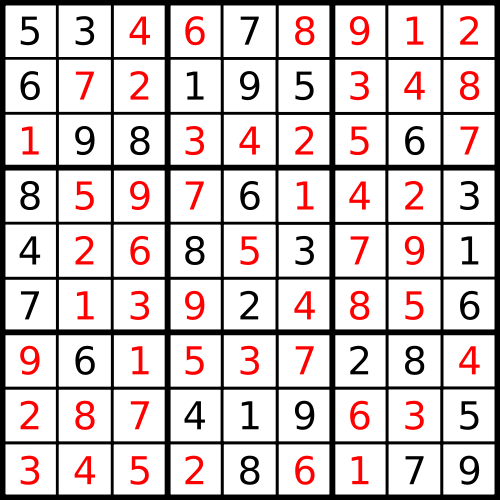
\includegraphics[width=45mm]{solved.png}}
	\caption{Solved 9x9 Sudoku Puzzle}
\end{center}
\end{figure}

Extending these rules to higher dimensions is fairly straightforward. The possible integers to be assigned to each row, column, and sub-grid becomes $[1,n]$.

In order to have a unique solution for a 9x9 grid, at least 17 starting numbers must be on the grid. While longed believed to be true, this was only proven two years ago.\footnote{\url{http://goo.gl/unmra}} As could be expected, then, the minimum number of starting numbers for higher dimensional grids is not readily computable. My program does not find all unique solutions, only the first that it encounters.

\section*{Algorithm Design}

\subsection*{Brute Force}

The most basic algorithm to compute the solution is a brute force algorithm. All possible solutions are created until the appropriate solution is found. Given that there are approximately $6.7 \times 10^{21}$ unique solutions for the 9x9 puzzle and 
an estimated $4.4\times10^{308}$ solutions for a 25x25 puzzle\footnote{\url{http://goo.gl/X9G5tV}}, this approach is incredibly inefficient. Even assuming we can solve 1000 puzzles per second (much faster than my optimized solution), it would take of on the order of $10^{11}$ years to compute the result for the 9x9 grid in the in the worst case (the 25x25 puzzle would take more years that there are baryons in the universe\footnote{\url{http://goo.gl/lTS4fO}} -- by a factor of more that $10^{200}$). My solution does not resort to this approach, but I though it useful to gain some sense of the efficiency gained from other techniques.


\subsection*{Backtracking}

An improvement upon the brute force approach is to implement a simple backtracking algorithm. This algorithm recursively traverses the tree of all possible solutions, only visiting children that put the puzzle closer to being solved. If a child of the current node is chosen that does not progress the solution, the change is undone and another path through a different child is attempted. That is, the algorithm \textit{backtracks} to the last valid state of the puzzle.

%diagram here
%insert solved sudoku grid here
\begin{figure}[h!]
\begin{center}
    \fbox{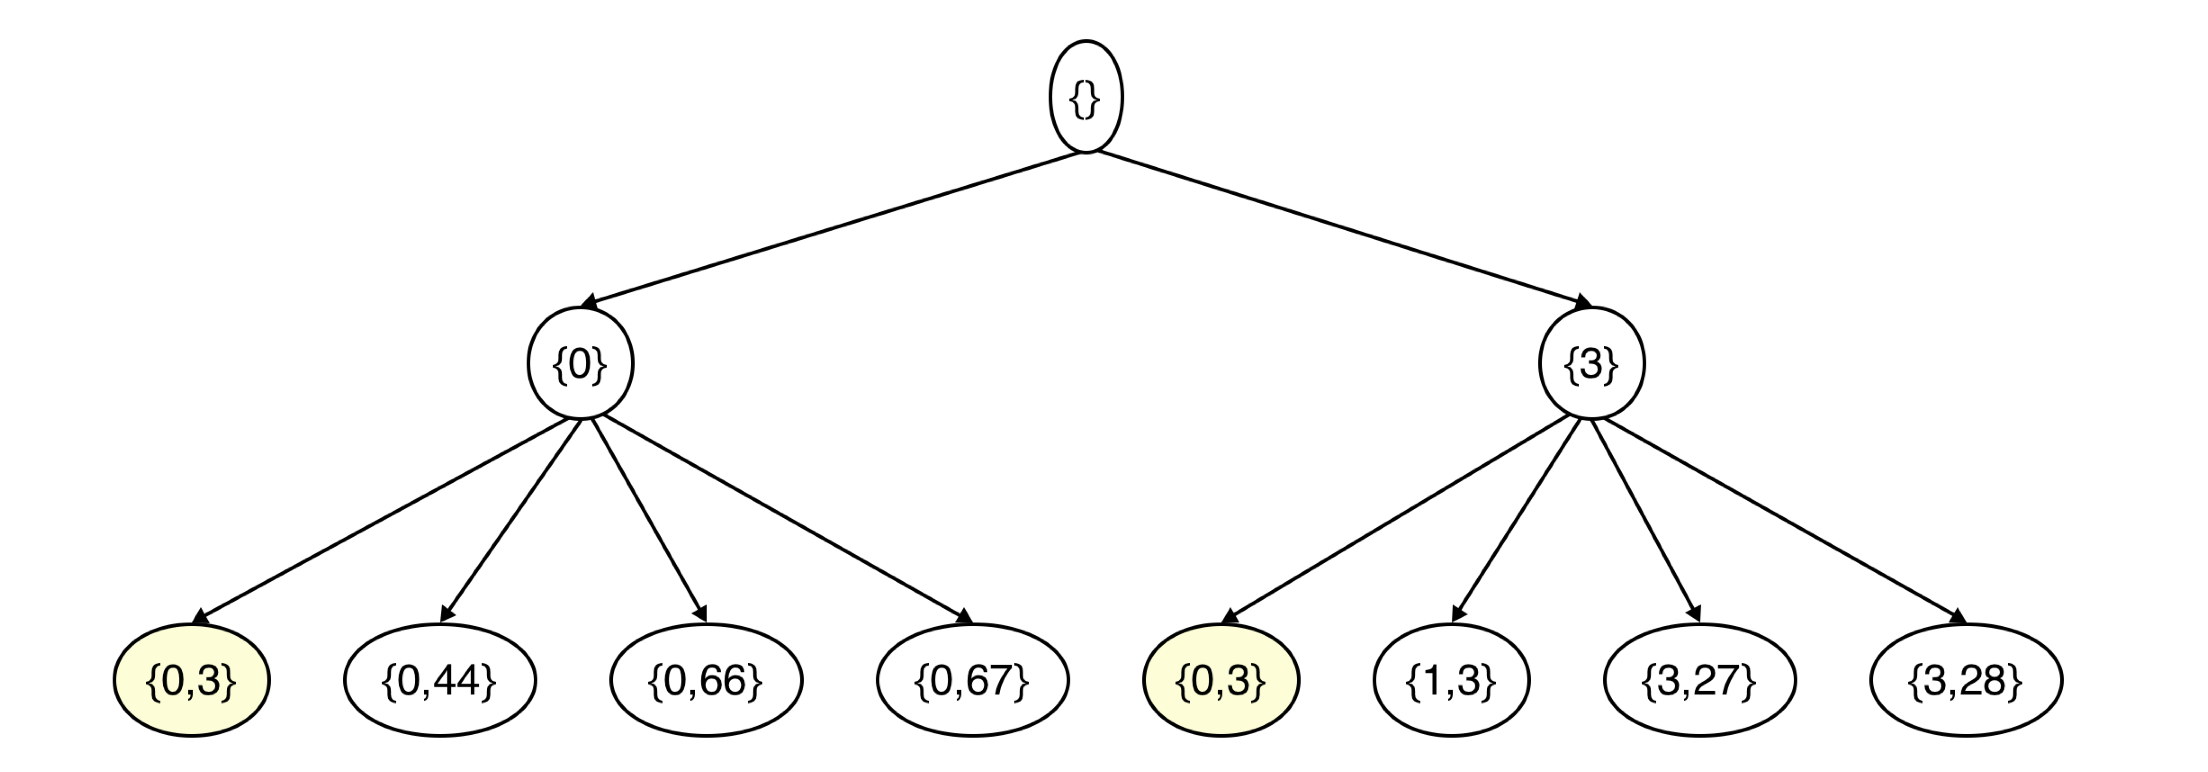
\includegraphics[width=130mm]{backtracking.png}}
	\caption{Simple Backtracking Tree}
\end{center}
\end{figure}

My program does utilize a backtracking search, but only when heuristic methods fail.

\subsection*{Forward Checking}

This technique is heuristic (is is also sometimes referred to as ``constraint propagation"). That is, it employs rules that more accurately model how a human would solve the puzzle. In doing so, the number of possible solutions can be greatly reduced before the backtracking search begins.

Before presenting my constraints, the following sets must be defined for some cell $c$.

\begin{itemize}[leftmargin=3cm]
	\item [\textbf{Peers:}] The set of all cells adjacent to $c$. These are cells in the immediate sub-square, row, and column.
	\item [\textbf{Units:}] This is the set (always of size 3) of the sets of values in the adjacent row, column and sub square. This includes $c$. 
	\item [\textbf{Values:}] All of the possible values for $c$.
\end{itemize}

Given the definitions, my two rules were

\begin{enumerate}[leftmargin=3cm]
	\item If a cell is reduced to one possible value (the starting squares, for instance), then this value cannot appear in any of its peers and is removed from their value sets. 
	\item If there is only one place for a value within a unit of $c$, then the value must be assigned there.
\end{enumerate}


Theses two rules were wrapped into an \texttt{assign(set values, digit d)} function. Before any backtracking takes place, this function is called to assign all of the given values to the board. Of course, the changes made as result of one value will almost always instigate further changes to the board (this is the ``propagation" in constraint propagation). When no more changes can be made, the backtracking search begins. Many easy puzzles are completely solved via this technique.

The backtracking search itself finds the cell with the fewest number of possible values and attempts to assign one of the remaining values to that cell via the same \texttt{assign} function (initiating the same ripple effect of constraints). If this function returns false, meaning the assignment could not be made, then the value of the Sudoku puzzle before the attempted assignment is restored. The same process is repeated until a value can be assigned to the cell. Eventually, all cells are assigned one value.

I should mention that I did attempt to implement other heuristic techniques, most notably the recognition of ``naked-twins." The strategy seeks to exploit the situation in which two cells of the same unit both have only the same two possible values. If this is the case, then the two values must be assigned to those two cells -- meaning they can be eliminated from all other cells in the unit. This is really just an extension of my first rule, and can be further generalized for higher order groupings (provided the number of cells in a unit is not exceeded).

I found, however, that implementing such a strategy did not speed up the 9x9 puzzle by much, and in many cases actually slowed it down -- there is significantly more overhead required to implement the logic of this rule. While someone with more programming chops could probably make it viable, this slowdown does show that there is certainly a point of diminishing returns in heuristic techniques.

\section*{Program Features}

My program was written in \texttt{C++} in an attempt to make it as fast as possible. In addition, the (in my opinion) excellent GUI toolkit FLTK is written in the same language. It will compile on any platform and is statically linked, making for a very small executable.

The program does not crash under any normal circumstances. It recognizes Sudoku puzzles that cannot be solved, and handles file exceptions appropriately. It will, however, run for an arbitrarily long time given a sufficiently complicated puzzle. There is no ``upper limit" to how long a computation will last. Most 5x5 puzzles tested, however, were solved within one minute (the majority were less than 10 seconds). Computation for smaller board sizes is nearly instantaneous. The ``hardest sudoku puzzle"\footnote{\url{http://goo.gl/cOr7jY}} is solved in about 150 ms on my Intel 2.3GHz Ivy-Bridge i7 quad.

\subsection*{Start Window}
The main window of my program directs the user to enter a manual editing mode or choose from a pre-encoded file. In addition, a selector is present to specify sub-square dimensions of the Sudoku board to either be edited or loaded. While the program will technically solve an arbitrarily large puzzle, a 36x36 grid does not fit onto most monitors. The selectable range is $[2,5]$.

%start window picture
\begin{figure}[h!]
\begin{center}
    \fbox{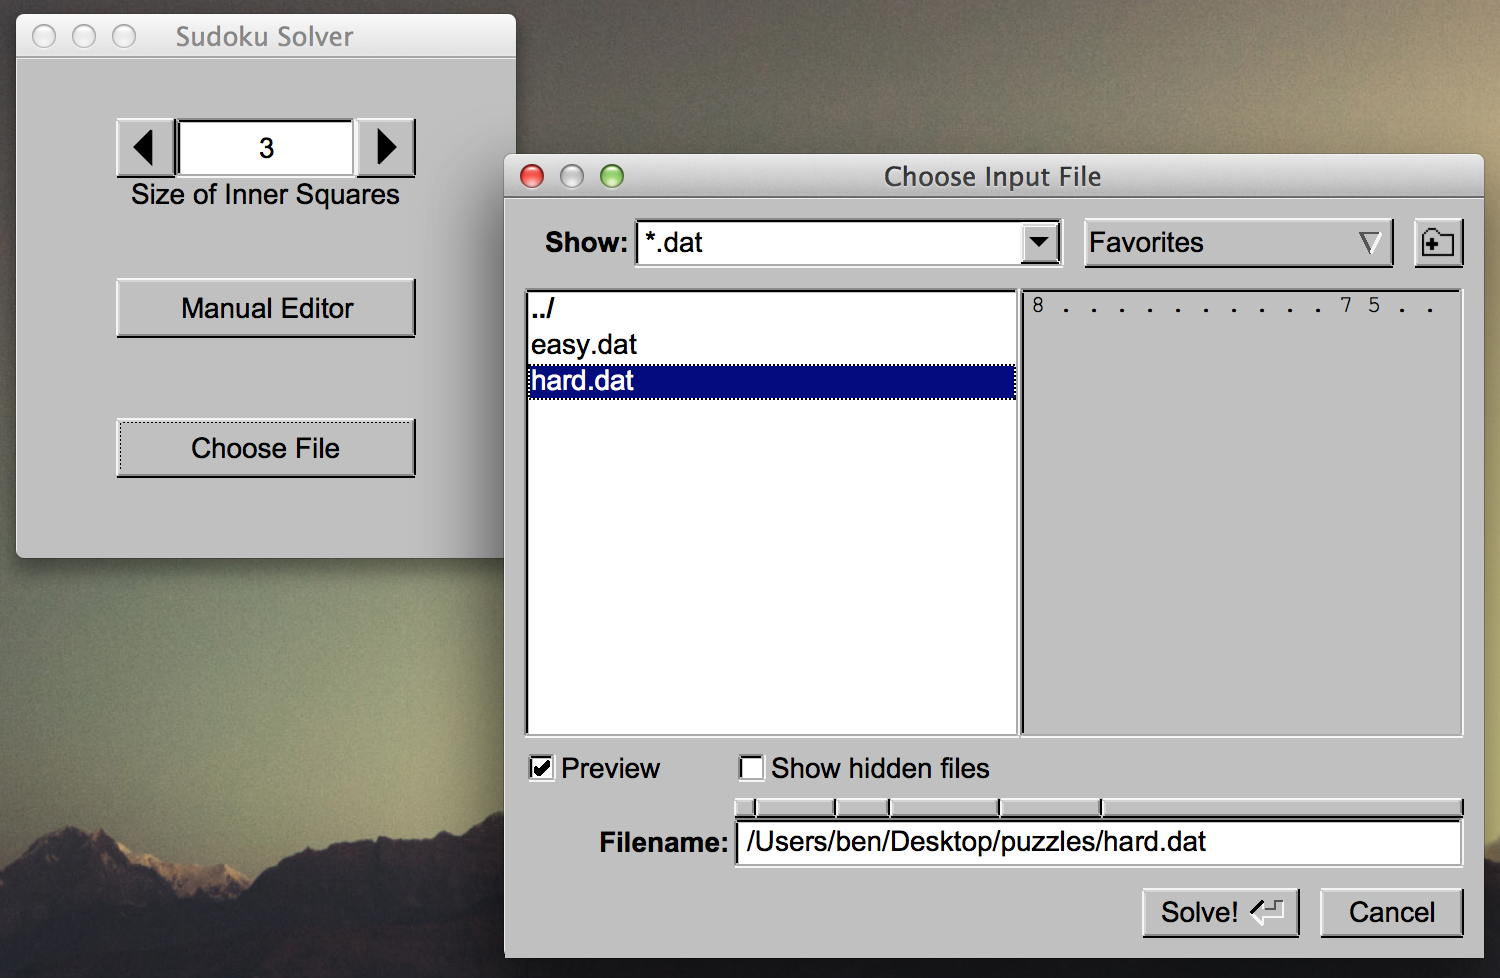
\includegraphics[width=100mm]{start.png}}
	\caption{Start Window}
\end{center}
\end{figure}

\subsection*{Editor}

The editor is a simple grid of input boxes that allow the user to input their puzzle. Only integer input within the allowed range is allowed, and the program will not launch if the grid is empty. In addition, the user is given the option to encode the current puzzle to a file.

%start window picture
\begin{figure}[h!]
\begin{center}
    \fbox{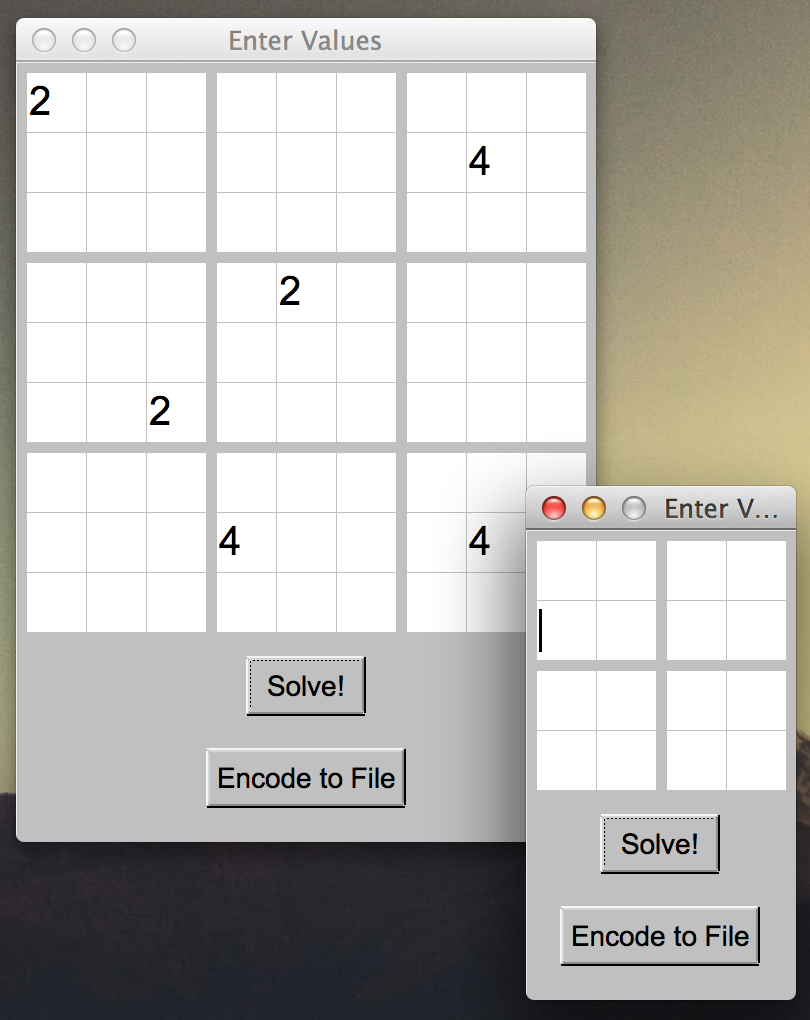
\includegraphics[width=50mm]{input.png}}
	\caption{Editor Window}
\end{center}
\end{figure}

\subsection*{Output}
The output window is structured similarly to the Editor window, with the obvious exception that the solution to the puzzle is shown. The solving time is also displayed at the bottom of the window.

\begin{figure}[h!]
\begin{center}
    \fbox{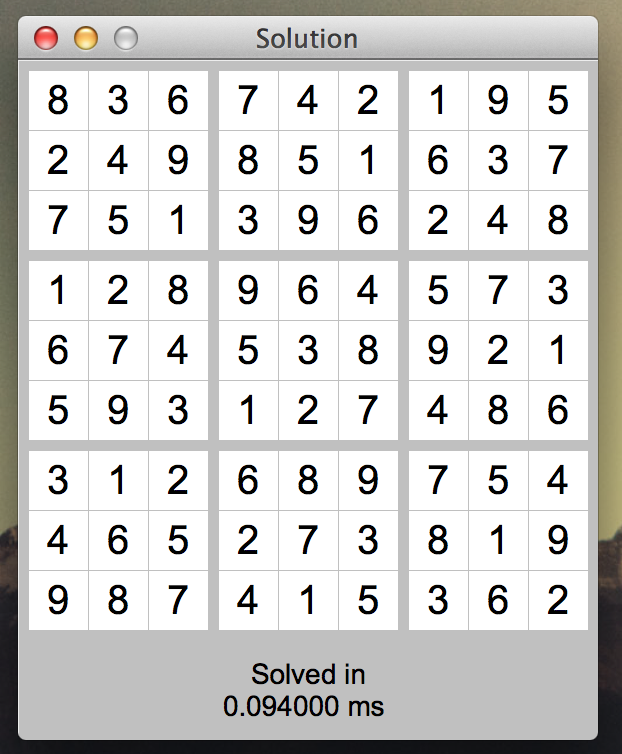
\includegraphics[width=60mm]{output.png}}
	\caption{Output Window}
\end{center}
\end{figure}


\end{document}
